\documentclass[12pt]{article}

% set indentation
\usepackage{parskip}
%\setlength{\parindent}{16mm}

% for the figures
\usepackage{graphicx}
\usepackage{extsizes}
\usepackage{wrapfig}
\usepackage{leftidx}
\usepackage{amsmath}
\usepackage{dsfont}
% change margins
\usepackage{geometry}
\geometry{left=20mm,right=20mm,top=15mm,bottom=15mm}

% for the reference
\usepackage[sort]{natbib}
\usepackage{url}
\usepackage{placeins}
%\usepackage{authblk}
\usepackage{setspace}
\usepackage{tabularx}
%\doublespacing
% in preamble
%\usepackage{movie15}
% in documenet

\usepackage{authblk}
\usepackage{graphicx}
% My packages
\usepackage{parskip}
\usepackage{relsize, threeparttable}
\usepackage{array}
\usepackage{booktabs}
\usepackage{lscape}
\usepackage{tabularx}
\usepackage{makecell}
\usepackage{booktabs}
\usepackage{numprint}
\usepackage{amsmath}
\usepackage{mathtools}
\usepackage{amssymb}
\usepackage{multirow}
\setlength{\parindent}{16mm}
% for the figures
\usepackage{graphicx}
\usepackage{placeins}
% for the reference
\usepackage{natbib}
\usepackage{floatrow}
\usepackage{chngcntr}
\usepackage{url}
\usepackage{dutchcal}
%\usepackage{boondox-calo}
\usepackage{upgreek}
%\date{}
\usepackage{color,soul}


\setlength{\parindent}{0pt}
\definecolor{lightgrey}{rgb}{0.925, 0.925, 0.925}
\sethlcolor{lightgrey}







\title{Unraveling the time dynamics of life annuities}

\author[1]{Jes\'us-Adri\'an \'Alvarez\thanks{jeal@atp.dk}}

\author[2]{Andr\'es M. Villegas}

\affil[1]{{\small No affiliation} }

\affil[2]{\small{School of Risk and Actuarial Studies and ARC Centre of Excellence in Population Ageing Research (CEPAR)\\ UNSW Business School, Sydney, Australia}}
%\date{}

\begin{document}
\maketitle

{
\setcounter{tocdepth}{2}
%\tableofcontents
}



\begin{abstract}
	
Mortality and interest rates evolve together, dynamically influencing life annuity values and reserves. This paper introduces differential equations that quantify the simultaneous impact of mortality and interest rate fluctuations on life annuities and reserves. The equations account for these fluctuations through entropies and durations, providing a clearer, more detailed view of life annuity risks and offering actionable insights for actuaries and risk managers.

Our framework explicitly captures the joint behavior of mortality and interest rates, enhancing the understanding of evolving economic-demographic environment. We demonstrate its utility using over 100 years of UK data, revealing how financial and longevity risks evolve at granular levels, such as age-term-specific contributions and causes of death. Our flexible, model-free equations empower practitioners to assess and manage the evolving risks in life annuity portfolios using real-world data.	
	
	
\end{abstract}
\newpage
\section{Introduction}\label{sec:1_introduction}
\section{Introduction}

Pension funds and insurance companies face increasing concerns about how simultaneous fluctuations in interest rates and mortality affect their life annuity portfolios. Two key uncertainties surround the time dynamics of life annuities. First, there is uncertainty about the future development of mortality and interest rates. Second, there is uncertainty about how life annuities (and their corresponding actuarial reserves and capital requirements) respond to changes in both mortality and interest rates. 

The first source of uncertainty has been studied extensively and a wide range of models to forecast mortality and interest rates have been proposed under many different perspectives. However, the second source—sensitivity of life annuities to fluctuations in mortality and interest rates—has been less explored. While much of the research on interest rate sensitivity has focused on immunization theory, studies on mortality sensitivity remain limited. An important contribution in this area comes from \citet{rabitti2020mortality}, who examined how mortality sensitivity varies with interest rates using historical life tables and assumed constant interest rates. Their findings suggest that mortality sensitivity is higher when interest rates are low, with the financial component becoming a key risk when both factors are considered.

\section{Introduction}

Pension funds and insurance companies are increasingly concerned with how simultaneous fluctuations in interest rates and mortality affect their life annuity portfolios. This concern is particularly relevant for high-income countries, which are currently experiencing rapid changes in interest rates and mortality improvements \citep{djeundje2022slowdown}, the latter of which were reversed by the COVID-19 pandemic \citep{aburto2022quantifying}. There are two primary sources of uncertainty regarding the time dynamics of life annuities. First, there is uncertainty about the future development of cohort mortality and interest rates. Second, there is uncertainty regarding how sensitive life annuities (and the corresponding reserves, capital charges, etc.) are to the simultaneous changes in mortality and interest rates. In other words, how do mortality and interest rates change over time, and how do life annuities respond to these changes?

The first source of uncertainty, namely forecasting mortality and interest rates, has been extensively studied. A wide range of statistical models have been proposed to forecast these variables from various perspectives \citep{cairns2017modelling,cairns2019modelling,kallestrup2020insight}. The second source of uncertainty, concerning the sensitivity of life annuities to changes in mortality and interest rates, has received less attention. Most studies on interest rate sensitivity have focused on immunization theory, while fewer studies have addressed mortality sensitivity.

A significant contribution in this regard is made by \citet{rabitti2020mortality}, who used model life tables for the United States in 1990 and for the United Kingdom (1990–1994), assuming different levels of constant interest rates. They found that mortality sensitivity was higher when interest rates were low (e.g., 0.5\%), whereas financial risk became more prominent when both sensitivities were considered together.

While the analysis by \citet{rabitti2020mortality} provides valuable insights into the joint sensitivities to mortality and interest rate changes, it remains unclear whether these results hold for different time periods or with real data on the term structure of interest rates. Furthermore, the speed at which sensitivities change over time and the sources of such changes (e.g., driving causes of death) remain unclear. Additionally, differences in age-specific mortality improvements and variations in the term-specific attributions of the yield curve may produce contrasting effects on life annuities. At present, there is no unified tool that can disentangle the effects of i) simultaneous fluctuations in mortality and interest rates, and ii) the sensitivity of life annuities, reserves, and risk measures to these fluctuations.

In this article, we introduce a set of differential equations to address the gap in understanding the time dynamics of life annuities and their associated reserves. Our approach quantifies the simultaneous contributions of changes in mortality and interest rates to these dynamics.

We begin by developing differential equations for a deterministic single life annuity factor. These equations are then expanded to disentangle the sources of change into age- and term-specific attributions and identifying the causes of death that drive these changes. Next, we generalize these equations to the stochastic representation of life annuity reserves, establishing the link with the well-known Thiele differential equation and discussing its applications in risk management. To illustrate the application of our framework, we analyze more than 100 years of data from the United Kingdom (1841–2016) to examine the long-term development of life annuity factors.


Our equations are simple, intuitive, and easily applicable, enabling actuaries and risk managers to assess the financial and longevity risks embedded in their life annuity portfolios using real data. From an actuarial perspective, these differential equations provide valuable insights for developing strategies to improve risk management, leveraging well-established concepts from mathematical demography and immunization theory.


The remainder of the article is structured as follows. In Section \ref{sec:SensitivityMortalityInterest}, we review key results from the actuarial and demographic literature on mortality and interest rate sensitivities. Section \ref{sec:TimeDynamics} presents the differential equations for the time dynamics of life annuities in the deterministic case. In Section \ref{sec:Reserves}, the equations are extended to the stochastic representation of annuity reserves. Section \ref{sec:UK_Illustration} illustrates the application of our equations using historical data from the United Kingdom. Lastly, we conclude with a discussion on the potential applications of the equations developed in this paper. The code to replicate the results and all derivations presented in this article are available in the open-source repository: \textit{link available upon publication}.



\section{Sensitivity to interest and mortality changes}\label{sec:SensitivityMortalityInterest}

\textit{\textbf{Duration}}

 Duration (hereafter denoted with variable $D$) is a fundamental quantity used to measure the effect of interest rates in any financial instrument. It is defined as the price sensitivity of a life annuity (or bond, fixed income, or any other financial instrument) to changes in the force of interest $\delta$ \citep{milevsky2013life,charupat2016sluggish}. Duration can be have different interpretations according to its application. For example, Macaulay duration estimates how many years it will take for an investor to be repaid the bond's price by its total cash flows. Modified duration measures the price change in a bond given a 1\% change in interest rates. Mathematically, duration is the first-order derivative of the financial quantity with respect to $\delta$, whereas the second-order derivative is given by the convexity. Both, duration and convexity are used in interest-rate immunization \citep{redington1951papers,fisher1971coping,shiu1990redington,santomero1997financial,courtois2007immunization} where portfolios are hedged against fluctuations in interest rates.


\textit{\textbf{Entropy}}


The entropy (hereafter denoted with variable $H$) is a measure that quantifies the sensitivity of a life expectancy to changes in death rates \citep{leser1955variations,keyfitz1977difference,demetrius1974demographic,goldman1986new,Vaupel1986}, such that higher the values of the entropy; the higher the sensitivity of life expectancy is to death rates. It has been shown that the entropy increases or decreases depending of the ages where mortality improvements take place \citep{aburto2019threshold}.

An important contribution in understanding the time dynamics of life expectancy via the entropy is done by \citet{Vaupel2003}. They show that the time derivative of life expectancy ($e(0,t)$) with respect to time $t$ can be expressed in terms of the general pace of mortality improvement ($\rho_{e}$) and the entropy ($H_{e}(t)$), such that:

\begin{equation}\label{eq:lifeexpdecomp}
	\dfrac{\partial e(0,t)}{\partial t}= \rho_{e}(t)H_{e}(t)e(0,t).
\end{equation}


Equation (\ref{eq:lifeexpdecomp}) clearly shows the changes over time in mortality and the sensitivity of life expectancy to these changes. This Equation allows further decomposition of age-specific and cause-specific contributions to mortality improvement and entropy.

\citet{Haberman2011} extended the concept of entropy to life annuities. In this context, the entropy measures the sensitivity of a life annuity to proportional changes in the force of mortality. The entropy of can be seen as an indicator longevity risk in ife annuity portfolios \citep{rabitti2020mortality}. \citet{alvarez2021linking} shows that it can be used to examine socio-economic disparities in pension systems.

There is a growing line of research that has used the entropy\footnote{with the name of mortality durations but it is essentially the same formulation as in \citet{Haberman2011}} in the context of mortality-immunization\footnote{similar to interest-immunization, mortality-immunization is defined as a set of strategies to ensure that the value of a portfolio will be little affected in response to changes in mortality rates}. In particular, \citet{wang2010optimal,tsai2011actuarial,Tsai2013a,Li2011} derive discrete formulas for life annuity entropies and convexities assuming constant and proportional changes in the force of mortality, $\mu$. Mortality-immunization has been applied to different types of life insurance and annuity products \citep{li2012key,Li2012,Wong2015,Luciano2015,levantesi2018natural}. 

\textit{\textbf{Bringing both perspectives together}}

Research regarding the sensitivity to mortality changes (mostly developed by demographers) and on sensitivity to interest rates (mostly developed by actuaries and financial managers) have remained largely disconnected\footnote{with exception of \citet{Haberman2011,rabitti2020mortality,alvarez2021linking} that made clear the links between both strands of research}. Paradoxically, both strands of research direct efforts at the same objective of study: gain a better understanding of the inherent sources of change in life contingent quantities.

Recently, \citet{Lin2020} made strides on this regard by deriving discrete formulas to calculate sensitivity of life annuities (and whole life insurances) to simultaneous changes mortality and interest rates. They introduced a synthetic variable called 'the force of mortality-interest`, which results from the addition of the force of mortality and interest ($\mu^*=\mu+\delta$). While the application of \citet{Lin2020} is interesting since it combines sensitivity in mortality and interest rates, it is unlikely that $\mu$ and $\delta$ change at the same pace over time. 

In this article we bring together the aforementioned results from the actuarial and demographic literature to the analysis of the time dynamics of life annuities. In the following section, we derive equations to this aim and describe their applications.

\section{Time dynamics of life annuities}\label{sec:TimeDynamics}
\subsection{Preliminaries}\label{preliminaries}

Let us introduce some notation about time variables used to describe the dynamics of life annuities. Let $(x)$ denote an insured life aged $x$, where $x>0$. The future lifetime of $(x)$ is denoted by random variable $S_x$. Therefore, $x+S_x$ is the random variable representing the lifetime of $(x)$, where time $S=s$ is the time variable associated to the \textit{development of the policy}.

The actuarial value of the policy associated to life $(x)$ is determined using information about the corresponding economic-demographic environment where the life annuity is written and provided. Let $T$ be the random variable representing the time when such information of \textit{the economic-demographic environment} is generated. We assume that this information is generated continuously, such that $T$ is continuous.

Time $t$ and $s$ are both time variables, however, they are not necessary the same. Information about the economic-demographic environment used to evaluate life annuities is indexed at time $t$. However, it could be that there is a lag between the time where the actuarial assumptions are set (at time $t$) and the time of development of the policy (denoted by time $s$). This is often the case of information regarding mortality rates which is collected by statistical offices at national with some years behind. In some cases it could be $t=s$, for example, some companies can have readily own experience data of the insured lives and market interest rates are also available continously. However, it is not always the case.

Here we decide to make a clear distinction between these two time variables with the purpose of unraveling the sources of change in life annuities\footnote{In Section \ref{sec:ThieleEquations} the link between $t$ and $s$ is analyzed explicitly in terms of the Thiele differential equation for a life annuity policy} and it will be useful in the derivation of the corresponding differential equations that portray such dynamics. In consequence, all of the quantities appearing in the remaining of the paper are indexed by $t$. 

\subsection{Changes over time $t$}

Let $I_{s,t}=\mathds{1}_{\{S_x>s,t\}}$ be the indicator of survival of life $(x)$ to time $s$, with information generated at time $t$. The expected value $\mathbb{E}[I_{s,t}]={}_sp_x(t)$ is the time $t$ period survival probability from age \(x\) to age \(x+s\), and ${}_sp_x(t)=e^{-\int_{0}^{s}\mu(x+y,t)dy}$, where \(\mu(x,t)\) is the force of mortality at age \(x\) in time $t$.

Let \(\delta(s,t)\) be the time $t$ forward force of interest at maturity $s$. This measure is a general form to express the term-structure of interest rates. Quantity ${v}(s,t)=e^{-\int_{0}^{s}\delta(y,t)dy}$ is the time $t$ discount factor for a cash-flow payable at maturity $s$.

In this article we use the convention that all derivatives with respect to time $t$ are denoted by adding a point on top of the quantity of interest. For example, time derivatives for the forces of mortality and interest are expressed as:

\begin{equation} \label{eq:mudot}
\dot{\mu}(x,t)\equiv\frac{\partial\mu(x,t)}{\partial t},
\end{equation}

and 

\begin{equation} \label{eq:mudot}
\dot{\delta}(s,t)\equiv\frac{\partial\delta(s,t)}{\partial t}.
\end{equation}

The rate of mortality improvement at age \(x\) and time $t$ is defined as

\begin{equation} \label{eq:rho}
\rho(x,t)=-\frac{\frac{\partial \mu(x,t)}{\partial t}}{\mu(x,t)} = - \frac{\dot{\mu}(x,t)}{\mu(x,t)}.
\end{equation}

Similarly, the relative change over time in the forward force of interest at maturity $s$ is defined as 

\begin{equation} \label{eq:phi}
\upvarphi(s,t)=-\frac{\frac{\partial \delta(s,t)}{\partial t}}{\delta(s,t)} = -\frac{\dot{\delta}(s,t)}{\delta(s,t)}.
\end{equation}

The actuarial present value of a continuous life annuity at age $x$ evaluated at time $t$ is given by

\begin{equation}\label{eq:Annuity}
\bar{a}_x(t) = \int_0^\infty {}_sp_x(t) {v}(s,t)ds = \int_0^\infty {}_sE_x(t) ds,
\end{equation}

where ${}_sE_x(t)={}_sp_x(t) {v}(s,t)$. 

A life annuity deferred $s$ years starting to be paid at age $x+s$ is expressed as

\begin{equation}\label{eq:DefAnnuity}
{}_s|\bar{a}_x(t) = {}_sE_x(t) \bar{a}_{x+s}(t).
\end{equation}


\subsection{Two types of changes: constant and proportional to $\mu$ and $\delta$}

We are interested in measuring changes in $\bar{a}_x(t)$ with respect to the time variable $t$. To achieve this aim, we first derive the corresponding expressions for durations and entropies associated to $\bar{a}_x(t)$. As mentioned in Section \ref{sec:SensitivityMortalityInterest}, the entropy of a life annuity captures changes in $\bar{a}_x(t)$ with respect to $\mu(x,t)$. The entropy of a life annuity issued for a life $(x)$ and evaluated at time $t$ is represented by ${H}_{x}(t)$. This quantity is denoted in general terms as:

\begin{equation}\label{eq:EntropyGeneral}
{H}_{x}(t) = \frac{ 1}{\bar{a}_x(t)}\cdot \frac{\partial \bar{a}_x(t) }{\partial \mu(x,t)}.
\end{equation}

Analogously, duration captures the sensitivity of $\bar{a}_x(t)$ to changes in interest rates. It is defined as the relative derivative of the annuity factor with respect to changes in the force of interest \citep{Milevsky2012,Milevsky2012a}:


\begin{equation}\label{eq:DurationGeneral}
{D}_{x}(t) = \frac{1}{\bar{a}_x(t)}\cdot  \frac{\partial \bar{a}_x(t) }{\partial \delta(s,t)}.
\end{equation}

Greater values for ${H}_{x}(t)$ and ${D}_{x}(t)$ indicate that $\bar{a}_x(t)$ is highly sensitive to changes in $\mu(x,t)$ and $\delta(s,t)$ respectively. The entropy and the duration can be determined by assuming the relationship between changes in in $\mu(x,t)$ and $\delta(s,t)$ relate to $\bar{a}_x(t)$. All formulations in the following sections are developing assuming constant (or parallel) and proportional movements in these quantities.

\textit{\textbf{{Changes in $\bar{a}_x(t)$ with respect to $\mu(x,t)$}}}

The entropy of a life annuity is denoted by ${H}^{c}_{x}(t)$ when changes in $\mu(x,t)$ are held constant at all ages and by ${H}^{p}_{x}(t)$ when changes are performed proportional. Based on the results developed by \citet{Tsai2013a} and \citet{Lin2020}, when $\mu(x,t)$ is changed constantly to $\mu(x,t)+\gamma$ such that $\gamma$ is a small number (see proof in Appendix), the entropy of $\bar{a}_x(t)$ becomes

\begin{equation}\label{eq:EntropyC}
{H}^{c}_{x}(t) = -\frac{\int_{0}^\infty s {}_sp_x(t) {v}(s,t) ds}{\bar{a}_x(t)}=\frac{{h}^{c}_{x}(t)}{\bar{a}_x(t)},
\end{equation}

where ${h}^{c}_{x}(t)=-\int_{0}^\infty s {}_sp_x(t) {v}(s,t) ds$. The term ${h}^{c}_{x}(t)$ is expressed in absolute (monetary) terms, whereas the entropy ${H}^{c}_{x}(t)$ is dimensionless because it does not depend on the absolute value of $\bar{a}_x(t)$.


\citet{Haberman2011} and \citet{Tsai2013a} show that when changes in $\mu(x,t)$ are assumed to be proportional to a small number $\gamma$ such that $\mu(x,t)(1+\gamma)$, the entropy of $\bar{a}_x(t)$ becomes

\begin{equation} \label{eq:EntropyP}
{H}^{p}_{x}(t) = -\frac{ \int_{0}^{\infty}{}_sp_x(t)\ln[{}_sp_x(t)] {v}(s,t) ds}{\int_0^\infty {}_sp_x(t) {v}(s,t) ds}.
\end{equation}


Alternatively, we show (see proof in Section \ref{sec:EntropyAlt} of the Appendix) that Equation (\ref{eq:EntropyP}) can be expressed as

\begin{equation} \label{eq:EntropyP2}
\begin{split}
{H}^{p}_{x}(t) &=  \frac{\int_0^\infty \mu(x+s,t)   {}_s|\bar{a}_x(t) ds}{\bar{a}_x(t)} =  \frac{{h}^{p}_{x}(t)}{\bar{a}_x(t)}, 
\end{split}
\end{equation}

where ${h}^{p}_{x}(t)=\int_0^\infty \mu(x+s,t)   {}_s|\bar{a}_x(t) ds$. Analogous to the case where changes are assumed to be constant, quantities ${h}^{p}_{x}(t)$ and ${H}^{p}_{x}(t)$ are expressed in absolute and relative terms respectively. The formulations shown in this section are closely related to the ones developed in the mortality-immunization literature \citep{Tsai2013a,Lin2020}. We extended them to the continuous case. 
 

\textbf{\textit{{Changes in $\bar{a}_x(t)$ with respect to $\delta(s,t)$}}}

 Similar to the entropy, changes in $\bar{a}_x(t)$ with respect to $\delta(s,t)$ can be assumed to be either constant or proportional. For the former case where changes are constant (or parallel), duration is expressed as:

\begin{equation}\label{eq:DurationC}
\begin{split}
{D}^{c}_x(t)&= -\frac{\int_0^\infty s {}_sp_x(t) {v}(s,t)ds}{\bar{a}_x(t)} \\
&= \frac{{d}^{c}_x(t)}{\bar{a}_x(t)},
\end{split}
\end{equation}

where ${d}^{c}_x(t)=-\int_0^\infty s {}_sp_x(t) {v}(s,t)ds$. Thus, assuming constant changes in $\delta(s,t)$ results into common types of duration known in finance as \textit{monetary duration}, ${d}^{c}_x(t)$, and \textit{modified duration}, ${D}^{c}_x(t)$ (see \citet{Milevsky2012} and \citet{Tsai2013a} for further details). It is worth noting that Equations (\ref{eq:EntropyC}) and (\ref{eq:DurationC}) are identical such that ${d}^{c}_x(t)={h}^{c}_{x}(t)$. Interestingly, this indicates that constant (i.e. parallel) changes in the force of mortality have essentially the same effect as parallel changes in the force of interest.


Assuming proportional changes in $\delta(s,t)$ (see proof in the Appendix) results in: 


\begin{equation}\label{eq:DurationP}
\begin{split}
{D}^{p}_{x}(t) &= -\frac{\int_0^\infty {}_sp_x(t) v(s,t) \ln(v(s,t))ds}{\bar{a}_x(t)}. \\
\end{split}
\end{equation}


Note that when assuming constant force of mortality such that $v(s,t)=e^{-\delta(t)s}$, we have that ${D}^{p}_{x}(t)=\delta(t){D}^{c}_{x}(t)$,


\begin{equation}\label{eq:DurationCP}
\begin{split}
{D}^{p}_{x}(t) &= -\frac{\int_0^\infty {}_sp_x(t) v(s,t) \ln(v(s,t))ds}  {\bar{a}_x(t)} \\
&=- \delta(t)\frac{\int_0^\infty s{}_sp_x(t) e^{-\delta(t)s}  ds}{\bar{a}_x(t)} \\
& = \delta(t){D}^{c}_{x}(t).
\end{split}
\end{equation}

Equation (\ref{eq:DurationP}) can also be re-expressed as:

\begin{equation}\label{eq:DurationP2}
\begin{split}
{D}^{p}_{x}(t) &= \frac{\int_0^\infty \delta(s,t) {}_s|\bar{a}_x(t)ds} {\bar{a}_x(t)} \\
                 &= \frac{{d}^{p}_{x}(t)}{\bar{a}_x(t)}.
\end{split}
\end{equation}


where ${d}^{p}_{x}(t)=\int_0^\infty \delta(s,t) {}_s|\bar{a}_x(t) ds$. 




\subsection{Time derivative of $\bar{a}_x(t)$} \label{sec:timderiv}

We now compute the derivative of $\bar{a}_x(t)$ with respect to the time variable $t$, $\dot{\bar{a}} _x(t)=\frac{\partial \bar{a}_x(t)}{\partial t}$, such that

\begin{equation}\label{eq:TimeDeriv}
\begin{split}
\dot{\bar{a}} _x(t) &= \int_0^\infty {}_s\dot{p}_x(t) v(s,t)ds +\int_0^\infty {}_sp_x(t) \dot{v}(s,t)ds.\\
\end{split}
\end{equation}


To develop a closed-form solution for Equation (\ref{eq:TimeDeriv}) we consider the general case where $_sp_x(t)=e^{-\int_{0}^{s}\mu(x+y,t)dy}$ and ${v}(s,t)=e^{-\int_{0}^{s}\delta(s,t)dy}$. We analyse separately each of the two terms in the right side of Equation (\ref{eq:TimeDeriv}). Let us first focus on the first term:


\begin{equation}\label{eq:TimeDerivP1}
\begin{split}
\int_0^\infty {}_s\dot{p}_x(t) v(s,t)ds &= \int_0^\infty   v(s,t) e^{-\int_0^{s}\dot{\mu}(x+y,t)dy}ds\\
&= -\int_0^\infty   v(s,t) {}_sp_x(t)\int_0^{s}\dot{\mu}(x+y,t)dyds\\
&= -\int_0^\infty  \dot{\mu}(x+s,t) \int_s^{\infty} v(y,t) {}_yp_x(t) dyds\\
&= - \int_0^\infty \dot{\mu}(x+s,t)   {}_sE_x(t) \bar{a} _{x+s}(t) ds\\
&= \int_0^\infty \rho(x+s,t) \mu(x+s,t)   {}_s|\bar{a}_x(t) ds.\\
\end{split}
\end{equation}


The second part equals:

\begin{equation}\label{eq:TimeDerivP2}
\begin{split}
\int_0^\infty {}_sp_x(t) \dot{v}(s,t)ds &= \int_0^\infty {}_sp_x(t)  e^{-\int_0^{s}\dot{\delta}(y,t)dy}ds\\
&= -\int_0^\infty {}_sp_x(t) v(s,t) \int_0^{s}\dot{\delta}(y,t)dy ds\\
&= -\int_0^\infty  \dot{\delta}(s,t)\int_s^{\infty} {}_yp_x(t) v(y,t) dy ds\\
&= \int_0^\infty  \upvarphi(s,t) \delta(s,t)  {}_s|\bar{a}_x(t) ds.\\
\end{split}
\end{equation}


Thus, $\dot{\bar{a}} _x(t)$ can be expressed as


\begin{equation}\label{eq:TimeDerivP3}
\begin{split}
\dot{\bar{a}}_{x}(t) &=  \int_0^\infty \rho(x+s,t) \mu(x+s,t){}_s|\bar{a}_x(t) ds +\int_0^\infty  \upvarphi(s,t) \delta(s,t)  {}_s|\bar{a}_x(t) ds\\
&= \int_0^\infty \rho(x+s,t) {}_sM_x(t)  ds +\int_0^\infty  \upvarphi(s,t) {}_sW_x(t)  ds,
\end{split}
\end{equation}


where ${}_sM_x(t)= \mu(x+s,t){}_s|\bar{a}_x(t)$ and ${}_sW_x(t)=\delta(s,t)  {}_s|\bar{a}_x(t)$. Dividing Equation (\ref{eq:TimeDerivP3}) by $\bar{a}_x(t)$ yields to:


\begin{equation}\label{eq:TimeDerivP}
\begin{split}
 \acute{\bar{a}}_x(t) = \frac{\dot{\bar{a}}_x(t)}{\bar{a}_x(t)}  = 
 \underbrace{\bar{\rho}_x(t){H}^{p}_x(t)}_\text{longevity component}
 +\underbrace{\bar{\upvarphi}(t){D}^{p}_x(t),}_\text{financial component}
\end{split}
\end{equation}

where $\bar{\rho}_x(t)= \frac{\int_0^\infty \rho(x+s,t) {}_sM_x(t)  ds}{\int_0^\infty  {}_sM_x(t)ds}$ and 
$\bar{\upvarphi}(t)= \frac{\int_0^\infty \upvarphi(s,t) {}_sW_x(t)  ds}{\int_0^\infty {}_sW_x(t) ds}$ are the weighted-average changes in mortality and interest rates respectively. Functions $\bar{\rho}_x(t)$ and $\bar{\upvarphi}(t)$ capture the stochastic change in the forces of mortality and interest whereas ${H}^{p}_x(t)$ and ${D}^{p}_x(t)$ capture the sensitivity due to changes in $\mu$ and $\delta$. In other words, Equation (\ref{eq:TimeDerivP}) entails that changes over time in annuity factors are driven by $\bar{\rho}_x(t)$ and $\bar{\upvarphi}(t)$, which are modulated by ${H}^{p}_x(t)$ and ${D}^{p}_x(t)$ respectively\footnote{Equation (\ref{eq:TimeDerivP}) can be seen as an extension of the Equation (\ref{eq:lifeexpdecomp}) developed by \citet{Vaupel2003} to measure changes over time in life expectancy}.


\subsection{Age and term contributions to changes in $\bar{a}_x(t)$}

Equation (\ref{eq:TimeDerivP}) gives a general way of understanding the sensitivity of the value of an annuity to overall changes in mortality and the term structure of interest rates. However, we may also be interested in understanding the contribution of particular age groups or specific terms of the yield curve to changes in the life annuity portfolio. This is in the spirit of the perfomance attribution exercises that are common in fixed income (see, e.g., \citet{Daul2012}).

 Let us define $n$ age groups $[x_{i-1}, x_i)$, $i=1,\ldots,n$, with $x_0=x$ and $x_n=\infty$, and $m$ term groups $[t_{j-1}, t_j)$, $j=1,\ldots,m$, with $t_0=0$ and $t_m=\infty$. Equation (\ref{eq:TimeDerivP3}) can be decomposed by age and term groups as follows:

\begin{equation}\label{eq:TimeDerivAge}
\begin{split}
 \acute{\bar{a}}_x(t) = \sum_{i=1}^n\int_{x_{i-1}-x}^{x_i-x}  \rho(x+s,t) {}_sM_x(t)  ds +\sum_{j=1}^m\int_{t_{j-1}}^{t_j}   \upvarphi(s,t) {}_sW_x(t)  ds.  
\end{split}
\end{equation}
We can also decompose the entropy $h_x^p(t)$ into $n$ age groups as follows:

\begin{equation} \label{eq:EntropyAge}
\begin{split}
{h}^{p}_{x}(t) &=  \sum_{i=1}^n\int_{x_{i-1}-x}^{x_i-x} \mu(x+s,t)   {}_s|\bar{a}_x(t) ds \\
&=  \sum_{i=1}^n {h}^{p}_{x}(t;x_{i_1},x_{i}),
\end{split}
\end{equation}
with ${h}^{p}_{x}(t;x_{i-1},x_{i})=\int_{x_{i-1}-x}^{x_i-x} \mu(x+s,t)   {}_s|\bar{a}_x(t) ds$, denoting the dollar entropy associated to proportional changes in the force of mortality between ages $x_{i-1}$ and $x_{i}$ and ${H}^{p}_{x}(t;x_{i-1},x_{i}) = \frac{{h}^{p}_{x}(t;x_{i-1},x_{i})}{\bar{a}_x(t)}$, the corresponding dimensionless entropy. 

Similarly, we can decompose the dollar duration $d^p(t)$ into $m$ term groups as follows:

\begin{equation}\label{eq:DurationAge}
\begin{split}
{d}^{p}_{x}(t) &= \sum_{j=1}^m\int_{t_{j-1}}^{t_j} \delta(s,t) {}_s|\bar{a}_x(t)ds \\
&= \sum_{j=1}^m {d}^{p}_{x}(t;t_{j-1},t_{j}),
\end{split}
\end{equation}

with ${d}^{p}_{x}(t;t_{j-1},t_{j}) = \int_{t_{j-1}}^{t_j} \delta(s,t) {}_s|\bar{a}_x(t)ds$, denoting the dollar duration associated to proportional changes in term structure between terms $t_{j-1}$ and $t_{j}$ and ${D}^{p}_{x}(t;t_{j-1},t_{j}) = \frac{{d}^{p}_{x}(t;t_{j-1},t_{j})}{\bar{a}_x(t)}$, the corresponding dimensionless duration. These age-specific entropies and term-specific durations are akin to the key q-durations \citep{li2012key} and key rate durations \citep{Ho1992}, which measure the sensitivity of financial instruments to changes in specific portions of the life table and term structure of interest rates.\\

Combining Equations (\ref{eq:TimeDerivAge}), (\ref{eq:EntropyAge}), (\ref{eq:DurationAge}):  

\begin{equation}\label{eq:TimeDerivAge2}
\begin{split}
 \acute{\bar{a}}_x(t) = \sum_{i=1}^n\bar{\rho}_x(t;x_{i-1}, x_i){H}^{p}_x(t;x_{i-1}, x_i) +\sum_{j=1}^m\bar{\upvarphi}(t;t_{j-1},t_{j}){D}^{p}_x(t;t_{j-1},t_{j}),  
\end{split}
\end{equation}
where $$\bar{\rho}_x(t;x_{i-1}, x_i)= \frac{\int_{x_{i-1}-x}^{x_i-x} \rho(x+s,t) {}_sM_x(t)  ds}{\int_{x_{i-1}-x}^{x_i-x}  {}_sM_x(t)ds}$$ and 
$$\bar{\upvarphi}(t;t_{j-1},t_{j})= \frac{\int_{t_{j-1}}^{t_{j}} \upvarphi(s,t) {}_sW_x(t)  ds}{\int_{t_{j-1}}^{t_{j}} {}_sW_x(t) ds}$$ are, respectively, the weighted average improvement rates in the age group $[x_{i-1},x_{i})$ and the weighted average pace of change in the force of interest for the term group $[t_{j-1},t_{j})$. 





\subsection{Cause of death decomposition}

Depending on the population, different causes of death can contribute substantially to the dynamics of the life annuity portfolio \citep{lin2005securitization,kallestrup2020insight}. A contemporary issue related to this pattern is the case of the excess mortality due to Covid-19 observed worldwide during the years 2020 and 2021 \citep{aburto2022quantifying}. To get insights about how causes of death shape the time dynamics of life annuities, the longevity component of Equation (\ref{eq:TimeDerivP}) can be easily decomposed into cause-specific contributions. 

Let ${_s}p{^i_x}(t)=e^{-\int_{0}^{s}\mu{^i}(x+y,t)dy}$ be the probability of surviving cause $i$ from age \(x\) to age \(x+s\) at time $t$, and $\mu{^i}(x+y,t)$ be the associated hazard. For $i=1,\dots,n$ independent causes of death, we have that ${_s}p{_x}(t)= \prod_{i=1}^{n} {_s}p{^i_x}(t)$. In this context, a whole life annuity can be expressed as $\bar{a}_x(t) = \int_0^\infty {_s}p{^1_x}(t) \cdots{_s}p{^n_x}(t) {v}(s,t)ds$. Deriving $\bar{a}_x(t)$ with respect to time $t$ yields to


\begin{equation}\label{eq:TimeDerivCoD}
\begin{split}
\dot{\bar{a}} _x(t) &= \int_0^\infty   {_s}\dot{p}{^1_x}(t) \cdots{_s}p{^n_x}(t) v(s,t)ds +\dots+\int_0^\infty   {_s}{p}{^1_x}(t) \cdots{_s}\dot{p}{^n_x}(t) v(s,t)ds +
\int_0^\infty {}_sp_x(t) \dot{v}(s,t)ds\\
&= \int_0^\infty  {_s}\acute{p}{^1_x}(t)  {_s}{p}{^1_x}(t) \cdots{_s}p{^n_x}(t) v(s,t)ds +\dots+\int_0^\infty   {_s}{p}{^1_x}(t) \cdots{_s}\acute{p}{^n_x}(t){_s}{p}{^n_x}(t) v(s,t)ds +\int_0^\infty {}_sp_x(t) \dot{v}(s,t)ds\\
&= \int_0^\infty  {_s}\acute{p}{^1_x}(t)  {_s}{p}{_x}(t)v(s,t)ds +\dots+\int_0^\infty   {}_s\acute{p}{^n_x}(t) {_s}{p}{_x}(t) v(s,t)ds +\int_0^\infty {}_sp_x(t) \dot{v}(s,t)ds\\
&= \sum_{i=1}^{n} \int_0^\infty  {_s}\acute{p}{^i_x}(t)  {_s}{p}{_x}(t)v(s,t)ds +\int_0^\infty {}_sp_x(t) \dot{v}(s,t)ds.
\end{split}
\end{equation}


Following the same procedure of Equation (\ref{eq:TimeDerivP1}), each component $\int_0^\infty  {_s}\acute{p}{^i_x}(t)  {_s}{p}{_x}(t)v(s,t)ds$ reduces to $\int_0^\infty  \rho^{i}(x+s,t){}_sM^{i}_x(t)ds$, where ${}_sM^{i}_x(t)= \mu^{i}(x+s,t){}_s|\bar{a}_x(t)$.  The last component of Equation (\ref{eq:TimeDerivCoD}) equals $\int_0^\infty  \upvarphi(s,t) {}_sW_x(t) ds$ as in Equation (\ref{eq:TimeDerivP3}). Thus, Equation (\ref{eq:TimeDerivCoD}) equals


\begin{equation}\label{eq:TimeDerivCoD2}
\begin{split}
\dot{\bar{a}} _x(t) &= \sum_{i=1}^{n} \int_0^\infty  \rho^{i}(x+s,t){}_sM^{i}_x(t)ds +\int_0^\infty  \upvarphi(s,t) {}_sW_x(t) ds.
\end{split}
\end{equation}

Dividing by $\bar{a} _x(t)$ we have


\begin{equation}\label{eq:TimeDerivCoD3}
\begin{split}
\acute{\bar{a}} _x(t) &= \sum_{i=1}^{n} \bar{\rho}{^i_x}(t){H}^{i}_x(t)+\bar{\upvarphi}(t){D}{^P_x}(t),
\end{split}
\end{equation}


where ${H}^{i}_x(t)=\dfrac{\int_{0}^{\infty}{}_sM^{i}_x(t)ds}{\bar{a} _x(t)}$ is the cause-specific entropy and $\bar{\rho}{^i_x}(t)=\dfrac{\int_{0}^{\infty}\rho{_x^i}(x+s,t) {}_sM^{i}_x(t)ds}{\int_{0}^{\infty}{}_sM^{i}_x(t)ds}$ is the average rate of mortality improvement of cause $i$.

\subsection{Assuming constant force of interest}


It is common that life annuities are computed by using a single interest rate, which represents the long-term expected return. Thus, $\acute{\bar{a}}_x(t)$ can be re-expressed by assuming a single interest rate $\delta(t)$ that varies over time $t$, such that $v(s,t)=e^{-\delta(t)s}$. This assumption affects the second part of Equation (\ref{eq:TimeDeriv}) as: 




\begin{equation}\label{eq:TimeDerivC1}
\begin{split}
\int_0^\infty {}_s{p}_x(t) \dot{v}(s,t)ds &=\int_0^\infty {}_s{p}_x(t) \frac{\partial \left[ e^{-\delta(t)s} \right]}{\partial t}ds \\
&=-\dot{\delta}(t)\int_0^\infty s  {}_s{p}_x(t) e^{-\delta(t)s} ds \\
&=  \dot{\delta}(t)  d^{c}_x(t).
\end{split}
\end{equation}

Substituting Equations (\ref{eq:TimeDerivP1}) and (\ref{eq:TimeDerivC1}) in Equation (\ref{eq:TimeDeriv}) results into: 


\begin{equation}\label{eq:TimeDerivC2}
\begin{split}
\acute{\bar{a}}_x(t) =  \bar{\rho}(t){H}^{p}_x(t)+\dot{\delta}(t)  D^{c}_x(t).
\end{split}
\end{equation}



Given that ${D}^{p}_{x}(t)=\delta(t){D}^{c}_{x}(t)$ (see Equation (\ref{eq:DurationCP})), it is straight-froward to show that in the case of a single interest rate, Equations (\ref{eq:TimeDerivP})  and (\ref{eq:TimeDerivC2}) are equivalent. Thus, it suffices to use the entropy (${H}^{p}_x(t)$) and the modified duration ($D^{c}_x(t)$) together with $\bar{\rho}(t)$ and $\dot{\delta}(t)$ to determine the contribution of financial and longevity risks to changes over time in life annuities.





\subsection{Recap of formulations}

Throughout Section \ref{sec:TimeDynamics}, we developed equations that can be used to determine the sources of change over time in life annuities. Overall, these equations comprise a financial component and a longevity component. Depending on the application, one can get insights about the age-specific and term-specific attribution of these components as well as cause-specific contributions. One can also make assumptions about the yield rate used in the calculations of life annuity portfolios. A summary of the equations introduced in this section is shown in the Table \ref{table:Table1}. 


\begin{table}[ht]
	\centering
	\begin{tabular}{lcc}
		\toprule
		\textbf{Description}&	\textbf{Financial component} & \textbf{Longevity component}   \\
		\hline
		\textit{General representation}&	$\bar{\upvarphi}(t){D}_x(t)$                           & $\bar{\rho}(t){H}_x(t)$ \\
		\hline
		\textit{Age-Term attributions}&	$\sum_{j=1}^m\bar{\upvarphi}(t;t_{j-1},t_{j}){D}_x(t;t_{j-1},t_{j})$                               & $\sum_{i=1}^n\bar{\rho}_x(t;x_{i-1}, x_i){H}^{p}_x(t;x_{i-1}, x_i)$ \\
		\hline
		\textit{Causes of death}&	$\bar{\upvarphi}(t){D}_x(t)$   & $\sum_{i=1}^{n} \bar{\rho}{^i_x}(t){H}^{i}_x(t)$ \\
		\hline
		\textit{Single interest rate}&	$\dot{\delta}(t){D}_x(t)$ & $\bar{\rho}(t){H}_x(t)$  \\
		\bottomrule
	\end{tabular}
	\caption{{Summary of expressions of the financial and longevity components used to determine the sources of change $\acute{a}_x(t)$}.}
	\label{table:Table1}
\end{table}



One of the main advantages of our framework is that the financial and longevity components are additive. Thus, the expressions in Table \ref{table:Table1} can be easily combined to get insights about the sources of change in $\acute{a}_x(t)$. For example, it can be the case that the actuary analysing fluctuations in the pension fund is interested in determining the term-specific contribution to the financial component as well as the causes of death that drive the longevity component. To this aim, the actuary can apply the equation $\acute{a}_x(t)=\sum_{j=1}^m\bar{\upvarphi}(t;t_{j-1},t_{j}){D}_x(t;t_{j-1},t_{j})+\sum_{i=1}^{n} \bar{\rho}{^i_x}(t){H}^{i}_x(t)$ to examine such dynamics. In the following section, we illustrate how our equations can be used using empirical data.



\FloatBarrier
\section{Time dynamics of reserves}\label{sec:Reserves}

In this section, we extend the previously derived equations to incorporate the stochastic representation of actuarial reserves.

Let a probability space be defined as $\{\Omega, \mathcal{F}, \mathbb{P}\}$, with \textbf{F} = $\{\mathcal{F}_t\}$ denoting a family of sub-$\sigma$-algebras that represents the information available at time $t$ about the economic-demographic environment. Recalling that $I_{s,t} = \mathds{1}_{\{S_x > s, t\}}$ and $\mathbb{E}[I_{s,t}] = {}_sp_x(t)$, we define a payment process $dB_t(s) = b(s) I_{s,t} \, ds$, where $b(s)$ is the continuous rate of benefit payments over the development of the policy for the insured life $(x)$.

Consider the policy value at maturity \( s \), evaluated based on information available at time \( t \), denoted as \({}_s\mathcal{V}_x(t)\). This is given by:
\[
{}_s\mathcal{V}_x(t) = \frac{1}{v(s, t)} \int_s^{\infty} v(y, t) \, dB_t(y),
\]
where \( v(s, t) \) represents the discount function from time \( t \) to \( s \), and \( B_t(y) \) is the accumulated benefit function at time \( t \) for benefit payment at \( y \). Notably, both mortality and interest rates are stochastic processes evaluated at time \( t \), as they are not deterministically known at time zero, i.e., at the time of policy issuance.. Given the requirement for the pension fund to maintain sufficient reserves to cover the financial value of \({}_s\mathcal{V}_x(t)\) at all times, the prospective reserve can then be expressed as:
\begin{equation}\label{eq:Reserve1}
	{}_sV_x(t) = \mathbb{E}[{}_s\mathcal{V}_x(t) \cdot v(s,t) \,|\, \mathcal{F}_t] = \mathbb{E} \left[ \int_s^\infty v(y,t) \, dB_t(y) \,|\, \mathcal{F}_t \right],
\end{equation}
which reduces to
\begin{equation}\label{eq:Reserve2}
	{}_sV_x(t) = \int_s^\infty v(y,t) \, {}_yp_x(t) \, b(y) \, dy.
\end{equation}

As in Section \ref{sec:TimeDynamics}, we differentiate Equation (\ref{eq:Reserve2}) with respect to time $t$:
\begin{equation}\label{eq:DifferentiateReserveT}
	{}_s\dot{V}_x(t) = \int_s^\infty \dot{v}(y,t) \, {}_yp_x(t) \, b(y) \, dy + \int_s^\infty v(y,t) \, {}_y\dot{p}_x(t) \, b(y) \, dy.
\end{equation}

Differentiating both sides of \ref{eq:DifferentiateReserveT} yields:
\begin{equation}\label{eq:DifferentiateReserveT2}
	\begin{split}
		{}_s\dot{V}_x(t) &= \int_s^\infty \upvarphi(y,t) \, \delta(y,t) \, {}_yV_x(t) \, dy + \int_s^\infty \rho(x+y,t) \, \mu(x+y,t) \, {}_yV_x(t) \, dy \\ 
		&= \int_s^\infty \upvarphi(y,t) \, {}_yW^V_x(t) \, dy + \int_s^\infty \rho(x+y,t) \, {}_yM^V_x(t) \, dy,
	\end{split}
\end{equation}
where ${}_yM^V_x(t) = \mu(x+y,t) \, {}_yV_x(t)$ is the attribution to mortality of the policy holder due to reaching age $(x+y)$, and ${}_yW^V_x(t) = \delta(y,t) \, {}_yV_x(t)$ is the interest earned on the amount of the reserve. Quantities $\rho(x+y,t)$ and $\upvarphi(y,t)$ denote changes at time $t$ in the demographic-economic environment where the reserve is evaluated. 


Similar to the deterministic case of a single annuity factor developed in Section \ref{sec:TimeDynamics}, we are interested in finding a closed expression for the relative change in the actuarial reserve, denoted by ${}_s\acute{V}_x(t)$. Dividing Equation (\ref{eq:DifferentiateReserveT2}) by ${}_sV_x(t)$ yields:
\begin{equation}\label{eq:AccuteDifferential}
	{}_s\acute{V}_x(t) = \underbrace{{}_s\bar{\rho}_x(t) \cdot {}_sH_x^V(t)}_\text{longevity component} + \underbrace{{}_s\bar{\upvarphi}(t) \cdot {}_sD_x^V(t)}_\text{financial component},
\end{equation}
where ${}_s\bar{\rho}_x(t) = \frac{\int_s^\infty \rho(x+y,t) \, {}_yM^V_x(t) \, dy}{\int_s^\infty {}_yM^V_x(t) \, dy}$ is the average change in mortality at all ages, and ${}_s\bar{\upvarphi}(t) = \frac{\int_s^\infty \upvarphi(y,t) \, {}_yW^V_x(t) \, dy}{\int_s^\infty {}_yW_x(t) \, dy}$ is the average term-structure change in interest rates over all terms. The sensitivities of the reserve to changes in mortality and interest rates are given by ${}_sH_x^V(t) = \dfrac{\int_{s}^{\infty} {}_yM^V_x(t) \, dy}{{}_sV_x(t)}$ and ${}_sD_x^V(t) = \dfrac{\int_{s}^{\infty} {}_yW^V_x(t) \, dy}{{}_sV_x(t)}$, respectively.

The differential equation (\ref{eq:AccuteDifferential}) decomposes changes in the reserve over time, where the effect of mortality improvements is modulated by the entropy, and changes in the term structure of interest rates are modulated by duration. Similar to the deterministic case of a single annuity factor, each term in Equation (\ref{eq:AccuteDifferential}) can be further decomposed into age-term attributions and cause-specific contributions, using the expressions from Table \ref{table:Table1}.


\subsection{Time dynamics over $s$ and over $t$}\label{sec:ThieleEquations}


Quantities $\mu$ and $\delta$ are not deterministically known at the time of policy issuance. Therefore, the actuarial valuation of the reserve ${}_sV_x(t)$ is done by the incorporation of assumptions (and models) that provide a reasonable depiction of the \textit{economic-demographic environment} where the policies operate. The differential equations (\ref{eq:DifferentiateReserveT2}) and (\ref{eq:AccuteDifferential}) capture the time dynamics of the reserve with respect to changes over time in the assumptions used for the actuarial valuation. These changes are indexed by time variable $t$.

On the other hand, changes in the reserve \({}_s\mathcal{V}_x(t)\) over the time horizon where the policy is in force (i.e. the \textit{policy term}) are described by the well-known \textit{Thiele's differential equation}. These changes are indexed by the time variable \( s \). Thiele's differential equation is a widely used tool for constructing reserves for life annuities within a market-consistent framework, as it captures the evolution of the reserve components over time.

 
Equation (\ref{eq:DifferentiateReserveT2}) and the Thiele's differential are closely related as they depict the dynamics of the reserve. This close relationship will be explored next.

The Thiele's differential equation for the reserve ${}_sV_x(t)$ is found by differentiating Equation (\ref{eq:Reserve2}) with respect to $s$:

\begin{equation}\label{eq:Thiele}
	\begin{split}
		\dfrac{\partial {}_sV_x(t)}{\partial s}&= \mu(x+s,t){}_sV_x(t) + \delta(s,t){}_sV_x(t) - b(s) \\
		&= {}_sM^V_x(t) + {}_sW^V_x(t) - b(s)
	\end{split}
\end{equation}

Then, ${}_sM^V_x(t)$ and ${}_sW^V_x(t)$ represent the quantities presented in Equation (\ref{eq:DifferentiateReserveT2}): ${}_sM^V_x(t) = \mu(x+s,t){}_sV(t)$, which represents the attribution to mortality of the policyholder due to reaching age $(x+s)$, and ${}_sW^V_x(t) = \delta(s,t){}_sV(t)$, which reflects the interest earned on the reserve amount ${}_sV(t)$. The quantity $b(s)$ denotes the rate of benefit payments, corresponding to the process $dB_t(s) = b(s) I_{s,t} \, ds$.

The attributions ${}_sM^V_x(t)$ and ${}_sW^V_x(t)$ are evaluated using the economic-demographic information available at time $t$. In the expression for ${}_s\dot{V}_x(t)$, shown in Equation (\ref{eq:DifferentiateReserveT2}), the attributions ${}_sM^V_x(t)$ and ${}_sW^V_x(t)$ are integrated over the remaining policy term $[s, \infty)$. This indicates that ${}_s\dot{V}_x(t)$ represents the total attribution of mortality and interest rates over the remaining policy term, accounting for changes in the economic-demographic assumptions at time $t$ (i.e., assumptions about interest rates and mortality). In other words, ${}_s\dot{V}_x(t)$ exclusively quantifies the time-$t$ developments in the actuarial assumptions at the policy time $s$.

 
The relationship between ${}_s\dot{V}_x(t)$ and the Thiele's differential equation becomes clearer when differentiating ${}_s\dot{V}_x(t)$ with respect to $s$: 

\begin{equation}\label{eq:DifferentiateVdotWithRespectS}
\dfrac{\partial	{}_s\dot{V}_x(t)}{\partial s}= \rho(x+s,t) {}_sM^V_x(t)+ \upvarphi(s,t) {}_sW^V_x(t)
\end{equation}

Equation (\ref{eq:DifferentiateVdotWithRespectS}) captures the change in the provision in two time dimensions: changes in the economic-demographic assumptions at time $t$, and at the development of the reserve at time $s$. 
Here the attributions ${}_sM^V_x(t)$ and ${}_sW^V_x(t)$ are modulated by the changes in mortality and interest rates via $\rho(x+s,t)$ and $\upvarphi(s,t)$.

Equation (\ref{eq:DifferentiateVdotWithRespectS}) extends the traditional Thiele’s differential equation by separating the sources of variation in the economic-demographic environment. Together with Equation (\ref{eq:DifferentiateReserveT2}), this equation has significant actuarial applications, such as in product development and risk management. Some of these applications, along with further developments, are discussed in the following section.



It is important to note that the rate of payment $b(s)$ no longer appears in Equation (\ref{eq:DifferentiateVdotWithRespectS}). This is because the benefit payments evolve solely over the development of the contract, i.e., over the period $[s, \infty)$, and do not depend on changes in the assumptions regarding the economic-demographic environment, i.e., changes at time $t$. This assumption is reasonable since benefit payments are typically adjusted over the length of the contract. However, this assumption can be modified, allowing for the possibility of using $b(s,t)$ instead.


Furthermore, it is possible that time $t$ and $s$ coincide, meaning that information about the economic-demographic environment is incorporated into the valuations at the same time the policy develops. However, in most cases, this is not necessarily true. In practice, a life insurance company or a pension fund may perform continuous evaluations of the actuarial provision using market-based yield curves, where financial information is continuously updated. In such cases, $t = s$ holds for interest rates. On the other hand, demographic statistics are typically published with some delay, and estimates of the force of mortality $\mu$ are made over broader time intervals. As a result, the experience of contract development at time $s$ often does not align with the pace at which demographic assumptions are updated at time $t$. Additionally, there may be value in distinguishing between times $t$ and $s$ in Scandinavian-style life insurance products, where it is common to differentiate between deterministic \textit{first-order} actuarial bases, prudently set by the actuary, and \textit{second-order} actuarial bases, which are usually based on market models.




\subsubsection{Risk management applications}

The differential equations developed in Section \ref{sec:Reserves} facilitate the analysis of risk drivers in the development of reserves, aligning with contemporary risk management practices.

For example, the current version of Solvency II regulations stipulates that a company must hold capital requirements for longevity risk corresponding to a shock that results in an immediate 20\% reduction in mortality rates across all ages. This shock can be represented by the factor $\bar{\rho} = 0.2$, which can then be used to determine the percentage impact on the reserve through the equation ${}_s\acute{V}_x(t) = {}_s\bar{\rho}_x(t) {}_sH_x^V(t) + {}_s\bar{\upvarphi}(t) {}_sD_x^V(t)$. Further scenario-based shocks to mortality and interest rates can be applied to ${}_s\acute{V}_x(t)$, where ${}_s\bar{\rho}_x(t)$ and $\bar{\upvarphi}$ are stressed. By utilizing the duration and entropy, actuaries and risk managers can leverage this tool to assess the impact of insurance and financial risks on their life annuity portfolios.

Along similar lines, ${}_s\bar{\rho}_x(t)$ and ${}_s\bar{\upvarphi}(t)$ can be modeled as stochastic processes adapted to a filtration \textbf{G} = $\{\mathcal{G}_t\}_{t \ge 0}$ such that ${}_s{\rho}^{\bf{G}}_x(t) = \mathbb{E}[{}_s\bar{\rho}_x(t) \mid \mathcal{G}_t]$ and ${}_s{\upvarphi}^{\bf{G}}(t) = \mathbb{E}[{}_s\bar{\upvarphi}(t) \mid \mathcal{G}_t]$. In this framework, the source of randomness in these stochastic processes can be explicitly modeled using forecasting models, enabling stochastic simulations. The resulting simulations of changes in reserves can then be used to calculate common risk metrics, such as VaR (Value at Risk), Expected Shortfall, and others. The ability to perform stochastic simulations of ${}_s{\rho}^{\bf{G}}_x(t)$ and ${}_s{\upvarphi}^{\bf{G}}(t)$ is particularly valuable in Asset-Liability modeling, where the impact of stochastic shocks on reserves is translated into corresponding management actions aimed at mitigating associated risks.

The risk analysis can be extended by examining the age-specific and term-specific stochastic variations in ${}_s{\rho}^{\bf{G}}_x(t)$ and ${}_s{\upvarphi}^{\bf{G}}(t)$, adapting the formulas presented in Table \ref{table:Table1}. These equations enable further segregation by sub-population, risk factors, or any cause of death.



\section{Historical changes in life annuities in the United Kingdom}\label{sec:UK_Illustration}

In this section we illustrate the formulations introduced in Section \ref{sec:TimeDynamics} by examining the sources of change in the long-term development of life annuities in the United Kingdom. We use two centuries of financial and demographic data, from 1841 to 2018. Age-specific mortality rates come from the \citep{HMD2020}, whereas long-term interest rates are represented by the yield on 2.5\% consols up to 2015, then by the yield of 20 year maturity bills (Bank of England, 2021 INSERT CITE IN .BIB FILE). We smoothed mortality and interest rates using splines \citep{green1993nonparametric,camarda2012mortalitysmooth} to obtain continuous estimates of the forces of mortality and interest respectively (Figure \ref{fig:Fig1}). Using our estimates of $\mu$ and $\delta$, we construct time series for life annuities at different ages and for both sexes. In this section we first focus on life annuity factors calculated for males at age 65, which represent a cut-off age for retirement in several populations. 


\begin{center}
	\textit{Figure 1 about here}
\end{center}




The upper panel of Figure \ref{fig:Fig2} depicts values for $\bar{a}_x(t)$ from 1841 to 2018 for males at age 65. We observe that during the second half of the 19th century and up to the decade of 1940s, $\bar{a}_{65}(t)$ remained at similar levels with small fluctuations. Thereafter, $\bar{a}_{65}(t)$ exhibited a sharp decline up to the decade of 1980s, followed by an increasing pattern that has remained until recent years. The lower panel of Figure \ref{fig:Fig2} show the relative derivative of $\bar{a}_{65}(t)$ with respect to time ($\acute{\bar{a}}_{65}(t)$). It is clear that $\acute{\bar{a}}_{65}(t)$ captures well the changes over time in life annuity; positive values indicate that $\bar{a}_{65}(t)$ goes up and negative values indicate a decrease in $\bar{a}_{65}(t)$. In the following sections we analyse the sources of change in the time trend of $\acute{\bar{a}}_{65}(t)$ by making use of the equations developed in Section \ref{sec:TimeDynamics}.


\begin{center}
	\textit{Figure 2 about here}
\end{center}


\subsection{Contribution of financial and longevity components to changes in $\bar{a}_x(t)$}

As shown in the formulas developed in Section \ref{sec:TimeDynamics}, changes over time in $\bar{a}_x(t)$ can be explained in terms of longevity and financial components. Each component depends on the time fluctuations of $\mu(x,t)$ and $\delta(s,t)$ (captured by $\bar{\rho}(t)$ and $\dot{\delta}(t)$ respectively) which are modulated by the sensitivity of $\bar{a}_x(t)$ to changes in the forces of mortality and interest (entropy, ${H}^{p}_x(t)$ and modified duration, ${D}^{c}_x(t)$). Figure \ref{fig:Fig3} depicts the components responsible of fluctuations over time in $\bar{a}_x(t)$.

\begin{center}
	\textit{Figure 3 about here}
\end{center}


The upper panel of Figure \ref{fig:Fig3} shows that between 1860 and 1940, there were some periods of mortality improvements and deterioration. However, as of the 1980s, $\bar{\rho}(t)$ increased steadily indicating an average mortality improvement between 2\% to 3\%. In recent years, $\bar{\rho}(t)$ trended downwards, which coincides with the mortality deterioration currently prevailing in the United Kingdom \citep{djeundje2022slowdown}. Regarding changes over time in the force of interest, we observe that $\dot{\delta}(t)$ has also remained at similar levels for most of the observation period with some fluctuations between 1930 and 1950. Since the 1960s, $\dot{\delta}(t)$ went up rapidly reaching the highest observed increase (of around 8\% in the decade of 1970s). Thereafter, $\dot{\delta}(t)$ declined faster and moved towards negative values entailing a decline in interest rates, which is still ongoing until recent time. Trends in $\bar{\rho}(t)$ and $\dot{\delta}(t)$ are responsible for the time trend we observe in $\bar{a}_x(t)$, which is modulated by the entropy, ${H}^{p}_x(t)$, and modifed duration, ${D}^{c}_x(t)$.


The lower panel of Figure \ref{fig:Fig3} shows that during most of the observation period, ${H}^{p}_x(t)$ was higher than ${D}^{c}_x(t)$. This indicates that $\bar{a}_x(t)$ has been more sensitive to changes in mortality than to changes in interest rates. However, these sensitivities have changed over time. The entropy show a decreasing trend that prevailed until to the 1980s. Modified duration, on the other hand, remained somewhat constant over time but as of the 1950s, it trended upwards reaching its maximum in the 1980s (of about 0.8). Thereafter, it decline again. It is worth noting that during some specific years, ${H}^{p}_x(t)$ and ${D}^{c}_x(t)$ depict the same values (i.e. in the 1960s). This means that during these years, $\bar{a}_x(t)$ was equally sensitive to changes in mortality and interest rates.




Using all the measures shown in Figure \ref{fig:Fig3}, we next calculate the contributions of financial ($\dot{\delta}(t){D}^{c}_x(t)$) and longevity risks ($\bar{\rho}(t){H}^{p}_x(t)$) to changes over time in $\bar{a}_{65}(t)$. The upper panel of Figure \ref{fig:Fig4} shows $\acute{\bar{a}}_{65}$\footnote{This is the same as Figure \ref{fig:Fig2}. We show it here so the reader can make sense of the decomposition} and the lower panel shows the financial and longevity components. Positive/negative values contribute to increase/decrease in $\bar{a}_x(t)$. From Figure \ref{fig:Fig4} it is clear that both, longevity and financial risks have played an important role in the long-term development of $\bar{a}_x(t)$. 

\begin{center}
	\textit{Figure 4 about here}
\end{center}

We can distinguish among four periods where life annuity factors fluctuated in response to specific changes in financial and longevity risks. From 1860 to 1945, stable annuity factors modulated by  contributions of longevity and financial components to the time trend. In a second period, from 1945 to 1970, we observe decreasing annuity factors mainly driven by the financial component. Around 1970, interest rates reached the highest point, which translated into a negative contribution of the financial component. In the next period, from 1970 to 2015, the time trend changed. Annuities went up due to positive contributions of both components. In the last period, from 2015 onwards, $\bar{a}_x(t)$ continue to increase with the longevity component contributing less to the trend. This reflects the deceleration of mortality improvements occurring in the United Kingdom and many other populations \cite{djeundje2022slowdown}.

\subsection{Attribution across age-groups and terms}

Next, we illustrate how the longevity and financial components in Figure \ref{fig:Fig4} can be further decomposed in age-term specific attributions. The yield curve used in this analysis was constructed using government bonds in the UK (commonly known as gilts) issued at different maturities. Data on gilts was retreived from the Bank of England (2021) and it covers the years 1970-2020.


Figure \ref{fig:Fig5} depicts the contribution of different age groups to the longevity component (i.e. ages 65-74,75-84, 85-94, 95-104) and terms in the yield curve (i.e. years 0-9, 10-19, 20-29, 30-39) from 1970 to 2018. At first glance, Figure \ref{fig:Fig5} reveals that the major contributions comes from ages 65-74 and interest rates with terms below 20 years. 

\begin{center}
	\textit{Figure 5 about here}
\end{center}

In Figure \ref{fig:Fig6}, we make a zoom into the age-term sensitivities for the years 1975 and 2015. The left panel shows that in 1975, durations and entropies for the 65-74 age group (i.e. terms 0-9 years) were much higher than in the other age-term groups. This indicates that annuities were highly sensitive to changes in mortality and interest in these ages-terms. However, in 2015 the picture changes, such that the entropy is much higher than the duration, but also the sensitivity to mortality improvements is more higher at ages between 75-94.

These findings are in stark contrast to the analysis carried out by \citet{rabitti2020mortality}, who argue that duration is the key driver in the total sensitivity. Indeed, Figure \ref{fig:Fig6} clearly shows that there is an interplay between interest and mortality and that both factors contribute substantially to the change in life annuities. 

\begin{center}
	\textit{Figure 6 about here}
\end{center}

\subsection{Cause of death contribution}

Finally, we dig into the causes of death that drive the longevity component. To this aim we obtain cause-specific death rates from the Human Cause-of-Death Database (HCD, INSERT REFERENCE IN BIB FILE) for the United Kingdom for the period 2001-2016. The causes are categorized using the ICD-10 international classification of diseases. For illustration purposes, we group  are six major causes of death used in the analysis: neoplasms (ICD-10 codes C00-D48), hearth diseases (ICD 10 codes I00-I52), cerebrovascular diseases (ICD-10 codes G45, I60-I69), respiratory diseases (ICD-10 codes J00-J22, J30-J98, U04) and other causes.

\begin{center}
	\textit{Figure 7 about here}
\end{center}

Figure \ref{fig:Fig7} depicts the cause-specific contributions to the longevity component for the years 2005, 2010 and 2015. Positive values indicate an increase in the longevity component while negative values indicate a reduction. In 2005, the main cause of death driving life annuity changes was heart diseases, followed by neoplasms and cardiovascular diseases and minor (but positive contributions) from respiratory diseases. This configuration changed substantially over time. In 2015, neoplasms were the main contribution to positive changes followed by heart diseases, whereas respiratory diseases and other causes of death contributed negatively to the change in longevity. EXPLAIN WHY IS IMPORTANT TO KNOW THESE SOURCES AND LINK THEM TO SOME STUDIES.


\section{Concluding remarks}\label{sec:6_Conclusion}

In this article, we introduced a set of differential equations that unravel the underlying sources of change in life annuities and their associated reserves. These equations are elegant, intuitive, and easily implementable with real-world data, representing a significant expansion of the mathematical toolkit available for pension and life insurance analysis.

The primary advantage of our approach lies in its ability to capture the simultaneous variation of mortality and interest rates. Our key equation reveals that changes in life annuities over time are driven not only by fluctuations in mortality and interest rates but also by their sensitivities to each of these factors, encapsulated by their entropies and durations.

Traditionally, actuaries and risk managers have monitored durations and entropies in isolation, often overlooking the interdependence between these indicators. However, in reality, mortality and interest rates evolve together over time, with durations and entropies adjusting dynamically to the changing economic-demographic environment. Although the correlation between mortality and interest rates remains an open question, both clearly influence the value of life annuities and reserves. Our differential equations explicitly account for this simultaneous behavior and the evolving sensitivities to mortality and interest rates.

Another key strength of the equations presented here is their flexibility. These model-free equations offer general expressions for the time dynamics of life annuities, avoiding the need for assumptions about the underlying demographic or economic environment. One of their most valuable applications is in monitoring the sources of change in life annuity portfolios using real data. To demonstrate this, we apply our framework to over 100 years of UK data, providing data-driven insights into the evolution of life annuity portfolios at various granular levels, such as age-term-specific contributions and causes of death.

While the primary focus of this article has been on the time dynamics of life annuities and reserves, the general framework we present is readily extendable to other life-contingent products. By incorporating lump sums, expenses, and more complex payment processes, future developments can expand the applicability of our approach.

A natural extension of our work is the adaptation of these equations to a multi-state Markov framework, where we can model intensities beyond mortality. This would enable the development of state-specific sensitivities, where variations in age-term intensities across different states could be explicitly accounted for.

Looking ahead, we anticipate that the differential equations developed in this paper will have broad applications in both actuarial practice and academic research. Regardless of the specific applications, the equations' ability to provide valuable insights into the time dynamics of life annuities ensures their continued relevance and utility in future developments.




\newpage

\bibliographystyle{apalike}
%\bibliography{/Users/Jesus/Documents/Papers/BibTex/Proposal}
%\bibliography{C:/Users/jmartinez/OneDrive - Syddansk Universitet/Papers/BibTeX/Proposal.bib}

\bibliography{library}

\newpage

\FloatBarrier
\section{Figures}

\begin{figure}[!ht]
	\centering
	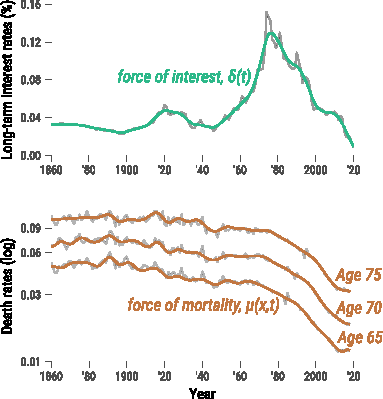
\includegraphics[width=0.5\linewidth]{Fig/deltamu}
	\caption{{Trends in interest and mortality rates calculated at ages 65, 70 and 75. Males, 1860-2018.}}
	\label{fig:Fig1}
\end{figure}


 \begin{figure}[!ht]
	\centering
	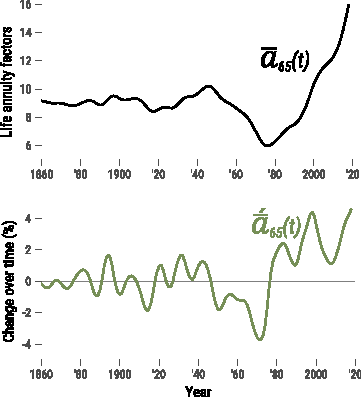
\includegraphics[width=0.5\linewidth]{Fig/axm}
	\caption{{Trends in life annuity factors and relative change in $\bar{a}_x(t)$ calculated at age 65. Males, 1860-2018.}}
	\label{fig:Fig2}
\end{figure}

\begin{figure}[!ht]
	\centering
	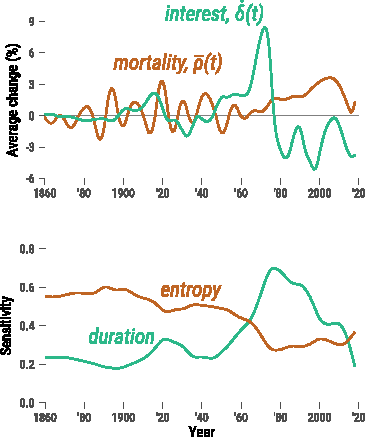
\includegraphics[width=0.5\linewidth]{Fig/IntMort}
	\caption{{Upper panel shows the average mortality improvement ($\bar{\rho}(t)$), and change in interest rates ($\dot{\delta}(t)$). Lower panel depicts the entropy ($H$) and modified duration ($D$). Males at age 65, 1860-2018.}}
	\label{fig:Fig3}
\end{figure}


\begin{figure}[!ht]
	\centering
	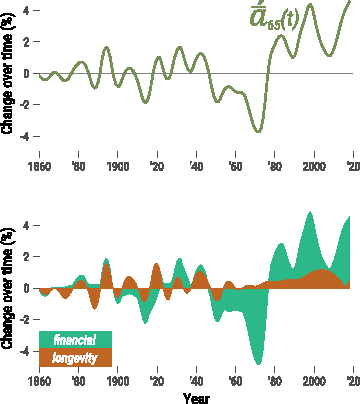
\includegraphics[width=0.5\linewidth]{Fig/DescSingle}
	\caption{{Decomposition of changes over time in life annuity factors calculated at ages 65. Males, 1860-2018.}}
	\label{fig:Fig4}
\end{figure}



\begin{figure}[!ht]
	\centering
	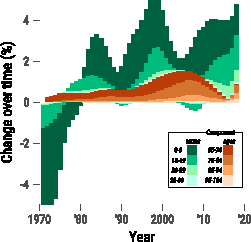
\includegraphics[width=0.4\linewidth]{Fig/DescAge}
	\caption{{Age and term attributions to changes over time in life annuity factors calculated at ages 65. Males, 1970-2018.}}
	\label{fig:Fig5}
\end{figure}


\begin{figure}[!ht]
	\centering
	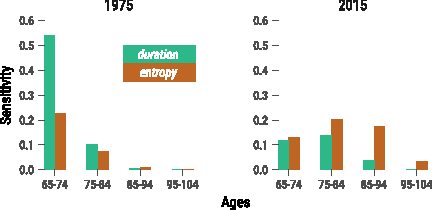
\includegraphics[width=0.7\linewidth]{Fig/AttributionDH}
	\caption{{Entropy and duration by age groups. Males, 1975 and 2015.}}
	\label{fig:Fig6}
\end{figure}

\begin{figure}[!ht]
	\centering
	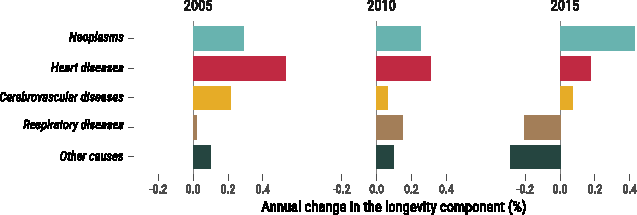
\includegraphics[width=1\linewidth]{Fig/DescCod}
	\caption{{Causes of death contributions to the changes in the longevity component. Males, 2005, 2010 and 2015.}}
	\label{fig:Fig7}
\end{figure}


\FloatBarrier
\newpage
\appendix
\section{Appendix}

\subsection{Entropy with constant changes in $\mu(x+s,t)$}\label{sec:EntropyConst}

To measure constant changes we make $\mu(s,t)+\gamma$, then

\begin{equation}\label{eq:EntropyConst1}
\begin{split}
\bar{a}_{x}(t) &= \int_0^\infty{v}(s,t) e^{-\int_{0}^{s} [\mu(x+y,t)+\gamma]dy}ds \\
&= \int_0^\infty {v}(s,t)e^{-\int_{0}^{s} \mu(x+y,t)dy} e^{-\gamma s}ds \\
&= \int_0^\infty {v}(s,t){}_sp_x(t) e^{-\gamma s}ds \\
\end{split}
\end{equation}

We expand $e^{-\gamma s}$ to $1-\gamma s+\frac{\gamma^2}{2} s^{2} +...$, so that


\begin{equation}\label{eq:EntropyConst2}
\begin{split}
\bar{a}_{x}(t) &= \int_0^\infty {}_sp_x(t) {v}(s,t)[1-\gamma s+\frac{\gamma^2}{2} s^{2} +...]ds
\end{split}
\end{equation}

We take the derivative $\bar{a}_{x}(t)$ with respect to $\gamma$ and evaluate $\gamma=0$


\begin{equation}\label{eq:EntropyConst3}
\begin{split}
{H}^{c}_x(t)&=\frac{1}{\bar{a}_x(t)}\frac{\partial \bar{a}_x(t)}{\partial \gamma} \bigg\rvert_{\gamma=0}\\
&= -\frac{\int_0^\infty s {}_sp_x(t) {v}(s,t)ds}{\bar{a}_x(t)} \\
&= \frac{{h}^{c}_x(t)}{\bar{a}_x(t)},
\end{split}
\end{equation}

where ${h}^{c}_x(t)=-\int_0^\infty s {}_sp_x(t) {v}(s,t)ds$



\subsection{Alternative expression for ${H}^{p}_{x}(t)$}\label{sec:EntropyAlt}

\begin{equation} \label{eq:EntropyAnnuityA1}
\begin{split}
{H}^{p}_{x}(t) &= -\frac{ \int_{0}^{\infty}{}_sp_x(t)\ln[{}_sp_x(t)] e^{-\int_{0}^{s}\delta(y,t)dy} ds}{\int_0^\infty {}_sp_x(t) e^{-\int_{0}^{s}\delta(y,t)dy} ds}\\
&= \frac{\int_0^\infty {}_sp_x(t) {v}(s,t) \int_0^s \mu(x+y,t) dy\,ds}{\bar{a}_x(t)}\\
&= \frac{\int_0^\infty  \mu(x+s,t) \int_s^\infty {}_yp_x(t) {v}(y,t)  dy\,ds}{\bar{a}_x(t)}\\
&= \frac{\int_0^\infty  \mu(x+s,t)  {}_sp_x(t) {v}(s,t) \int_s^\infty \frac{ {}_yp_x(t) {v}(y,t)}{ {}_sp_x(t) {v}(s,t)}  dy\,ds}{\bar{a}_x(t)}\\
&=  \frac{\int_0^\infty \mu(x+s,t)   {}_sp_x(t) {v}(s,t) \bar{a}_{x+s}(t) ds}{\bar{a}_x(t)} \\
&=  \frac{\int_0^\infty \mu(x+s,t)  {}_s|\bar{a}_x(t) ds}{\bar{a}_x(t)} \\
&=  \frac{{h}^{p}_{x}(t)}{\bar{a}_x(t)}, \\
\end{split}
\end{equation}

where ${h}^{p}_{x}(t)=\int_0^\infty \mu(x+s,t)   {}_s|\bar{a}_x(t) ds$.



\subsection{Duration with constant changes in $\delta(s,t)$}\label{sec:DurConst}

To measure constant changes we make $\delta(s,t)+\gamma$, then

\begin{equation}\label{eq:DurationConst1}
\begin{split}
\bar{a}_{x}(t) &= \int_0^\infty {}_sp_x(t) e^{- \int_{0}^{s} [\delta(y,t)+\gamma]dy}ds \\
&= \int_0^\infty {}_sp_x(t) e^{- \int_{0}^{s}\delta(y,t)dy}e^{-\gamma s}ds \\
&= \int_0^\infty {}_sp_x(t) {v}(s,t)e^{-\gamma s}ds
\end{split}
\end{equation}

We expand $e^{-\gamma s}$ to $1-\gamma s+\frac{\gamma^2}{2} s^{2} +...$, so that


\begin{equation}\label{eq:DurationConst1}
\begin{split}
\bar{a}_{x}(t) &= \int_0^\infty {}_sp_x(t) {v}(s,t)[1-\gamma s+\frac{\gamma^2}{2} s^{2} +...]ds
\end{split}
\end{equation}

We take the derivative $\bar{a}_{x}(t)$ with respect to $\gamma$ and evaluate $\gamma=0$


\begin{equation}\label{eq:DurationConst2}
\begin{split}
{D}^{c}_x(t)&=-\frac{1}{\bar{a}_x(t)}\frac{\partial \bar{a}_x(t)}{\partial \gamma} \bigg\rvert_{\gamma=0}\\
              &= \frac{\int_0^\infty s {}_sp_x(t) {v}(s,t)ds}{\bar{a}_x(t)} \\
              &= \frac{{d}^{c}_x(t)}{\bar{a}_x(t)},
\end{split}
\end{equation}

where ${d}^{c}_x(t)=\int_0^\infty s {}_sp_x(t) {v}(s,t)ds$



\subsection{Duration with proportional changes in $\delta(s,t)$} \label{sec:DurProp}

To calculate duration with proportional changes in $\delta(s,t)$, we assume that $\gamma$ is a small number such that $\delta(s,t)(1+\gamma)$ and  ${v}(s,t)=e^{-\int_0^{s}  \delta(y,t)(1+\gamma)dy}$.


\begin{equation}\label{eq:DurationProp1}
\begin{split}
\bar{a} _x(t) &= \int_0^\infty {}_sp_x(t) e^{-\int_0^{s}\delta(y,t)(1+\gamma)dy}ds \\
&= \int_0^\infty {}_sp_x(t) e^{-\int_0^{s}\delta(y,t)dy}e^{-\int_0^{s}\delta(y,t)\gamma dy}ds \\
&= \int_0^\infty {}_sp_x(t) v(s,t)v(s,t)^{\gamma}ds \\
\end{split}
\end{equation}


We expand $v(s,t)^{\gamma}$ to $1+\ln(v(s,t)) \gamma+{\ln(v(s,t))}^2 \frac{\gamma^2}{2}+...$, so that


\begin{equation}\label{eq:DurationProp2}
\begin{split}
\bar{a}_x(t) &= \int_0^\infty {}_sp_x(t) s(y,t)[1+\ln(v(s,t)) \gamma+{\ln(v(s,t))}^2 \frac{\gamma^2}{2}+...]ds\\
\end{split}
\end{equation}


To calculate the duration ${D}^{p}_{x}(t)$ we take the derivate of the expression above with respect to $\gamma$ and make $\gamma=0$

\begin{equation}\label{eq:DurationProp3}
\begin{split}
{D}^{p}_{x}(t)&=-\frac{1}{\bar{a}_x(t)}\frac{\partial \bar{a}_x(t)}{\partial \gamma} \bigg\rvert_{\gamma=0} \\
&= -\frac{\int_0^\infty {}_sp_x(t) v(s,t) \ln(v(s,t))ds}{\bar{a}_x(t)} \\
\end{split}
\end{equation}


Equation \ref{eq:DurationProp3} can be re-expressed as 


\begin{equation}\label{eq:DurationProp4}
\begin{split}
{D}^{p}_{x}(t) &= -\frac{\int_0^\infty {}_sp_x(t) v(s,t) \ln(v(s,t))ds}{\bar{a}_x(t)}\\
&= \frac{\int_0^\infty {}_sp_x(t) v(s,t) \int_0^{s} \delta(y,t)dy ds }{\bar{a}_x(t)}\\
&= \frac{\int_0^\infty \delta(s,t)  \int_{s}^{\infty} {}_{y}p_x(t) v(y,t)dy ds }{\bar{a}_x(t)}\\
&= \frac{\int_0^\infty \delta(s,t) {}_sp_x(t) v(s,t) \bar{a}_{x+s}(t)  ds }{\bar{a}_x(t)}\\
&= \frac{\int_0^\infty \delta(s,t) {}_s|\bar{a}_x(t) ds}{\bar{a}_x(t)} \\
&= \frac{{d}^{p}_{x}(t)}{\bar{a}_x(t)}.
\end{split}
\end{equation}



where ${d}^{p}_{x}(t)=\int_0^\infty \delta(s,t) {}_s|\bar{a}_x(t) ds$.




\end{document}
